\documentclass{IEEEtran}
\usepackage{cite}
\usepackage{amsmath,amssymb,amsfonts}
\usepackage{algorithmic}
\usepackage{graphicx}
\usepackage{textcomp}
\usepackage{caption}
\usepackage{fontenc}

\def\BibTeX{{\rm B\kern-.05em{\sc i\kern-.025em b}\kern-.08em
    T\kern-.1667em\lower.7ex\hbox{E}\kern-.125emX}}
\begin{document}
\title{Design and Implementation of an Elliptic Curve Arithmetic Unit}

\author{Melvin Bosjnak Jr's Jr.., Dan ``The Man'' Humeniuk, and Sir Jaden Simon III}

\maketitle

\begin{abstract}

Our group designed and implemented a 7-bit Elliptic Curve Arithmetic Unit which can multiply a point on an elliptic curve with a scalar. Elliptic-curve computations are expensive in software and thus the goal was to create a hardware implementation. This design is a proof-of-concept and would be need to be scaled up and generalized to be apart of a larger system. 

\end{abstract}

\begin{IEEEkeywords}
Elliptic curve cryptography, modulo multiplication, Mastrovito multiplier

\end{IEEEkeywords}

\section{Introduction}

Cryptography is a major component of computer security and comprises a large portion of computations required by devices. Elliptic-curve cryptography (ECC) uses many floating-point division operations in software, requiring a huge amount of time to complete. Hardware acceleration seems like a good solution to this problem, freeing up processor time to be spent on other tasks. Our Elliptic Curve Arithmetic Unit (ECAU) serves as a proof-of-concept to be apart of a larger ECC system. ECC requires a couple key operations over elliptic curves: point addition and point-scalar multiplication. The ECAU implements point-addition and thereby point-scalar multiplication.

Elliptic curves come in two forms: binary and prime. The binary curve works with binary extension fields and the prime curve works with prime fields. We chose to focus on the binary curve, primarily because the prime field is much harder to work on in hardware. In the binary field $\mathbb{F}_2$ there are only two elements: 0 and 1. To represent more elements, we can define a polynomial $P(x)$ whereby there is some number $\alpha$ that is a solution to $P=0$. If $P(x)$ is irreducible and of degree $m$, then elements within the field $\mathbb{F}_{2^m}$ can be represented as an $m-1$ degree polynomial: $a_{m-1}\alpha^{m-1} + a_1\alpha^{m-2} + ... + a_{0}$ where $a_{i} \in \mathbb{F}_2$. Notice that $m$-bit binary words are also elements within the field, each bit corresponding to an $a_{i}$. In order to create closure within the field, any operation done with the elements must be done modulo $P(x)$. Points on our curve are then a 2-tuple: $(x, y)$ where $x, y \in \mathbb{F}_{2^m}$.

\section{Implementation}

To keep things simple, we restricted our design to 7-bits. This means working over the finite field with 128 elements $\mathbb{F}_{2^7}$ using the primitive polynomial $P(x) = x^7 + x + 1$. All operations done with elements in the finite field will need to be done modulo $P(x)$. A total of 37 IO pins were needed, 28 for the input/output point, 7 for the scalar, and 2 for control signals. 

% Block diagram here
\begin{figure}%[H]
\centering
\captionsetup{justification=centering}
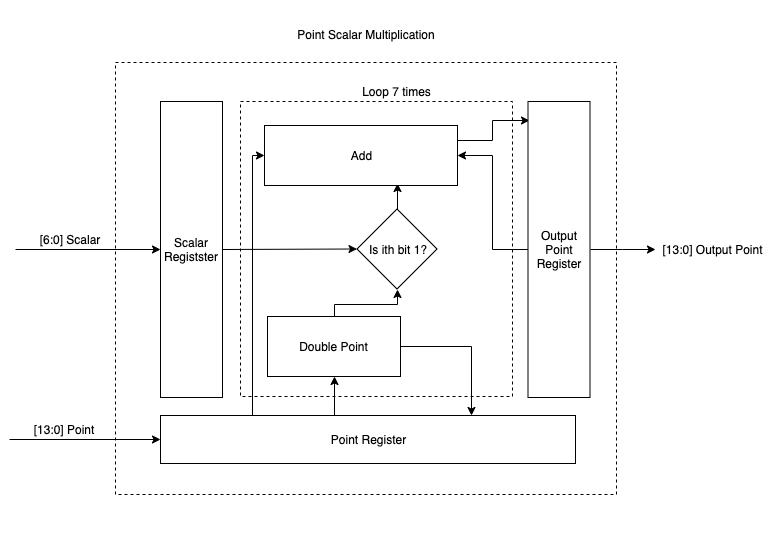
\includegraphics[width=0.5\textwidth]{images/blockdiagram.png}
\caption{Block diagram of our implemented ECAU}
\label{block}
\end{figure}

Before computations over curves can be performed, primitive operations such as multiplication, addition, and inversion of finite field elements must be implemented. Addition is easily implemented as bitwise XOR because the characteristic of the field is 2, while multiplication was done through a combinational Mastrovito multiplier \cite{Kallabook}. We were able to perform formal verification of the Mastrovito multiplier circuit with the use of Singular. The specification of the circuit $Z=A*B$ was compared with the netlists for the circuit. Each polynomial in the netlist as well as the specification were instantiated an ideal which is a special subset of our ring. The computed the Gr{\H o}bner basis of the ideal resulted in 1 which proved that the Mastrovito multiplier was correct. For inversion, we implemented the extended binary GCD algorithm. This is by far the most expensive operation, future work would focus on optimizing the inversion operation.

With the primitive operations done, we can now use equations derived from the Koblitz curve to perform point addition. Doubling a point is the same thing as adding a point to itself, using the tangent to the curve in place of the slope. Point-scalar multiplication was done with the classic double-and-add algorithm commonly used in integer multiplication. Our final FSM uses a reset signal to begin the computation, then sets a done flag when the output is ready. 

\section{Synthesis}

Once our verilog code was complete, we selected our top module and synthesized the design. We ran the synthesized design in Synopsys DC. This gave us the mapped verilog file. IO Pads, as mentioned in Section II, were added to the top module. We ran a rlace and route script in Innovus to implement the design to a physical chip. Once we had a GDS file from the Place and Route stage, we imported the design into Virtuoso. In Virtuoso, we added a seal ring to the design. From here we ran the DRC and LVS design checks on our design. We then ran poly fill and metal fill on the design (some fills may not have actually happened). The chip was finalized in Virtuoso and the result can be seen in Figure \ref{chip}. All steps of the process were simulated in Modelsim, giving a waveform as seen in \ref{sim}. In this specific case, multiplying the point (119, 65) by 72 results in the same point as expected by our testing scripts.

% Chip here
\begin{figure}%[H]
\centering
\captionsetup{justification=centering}
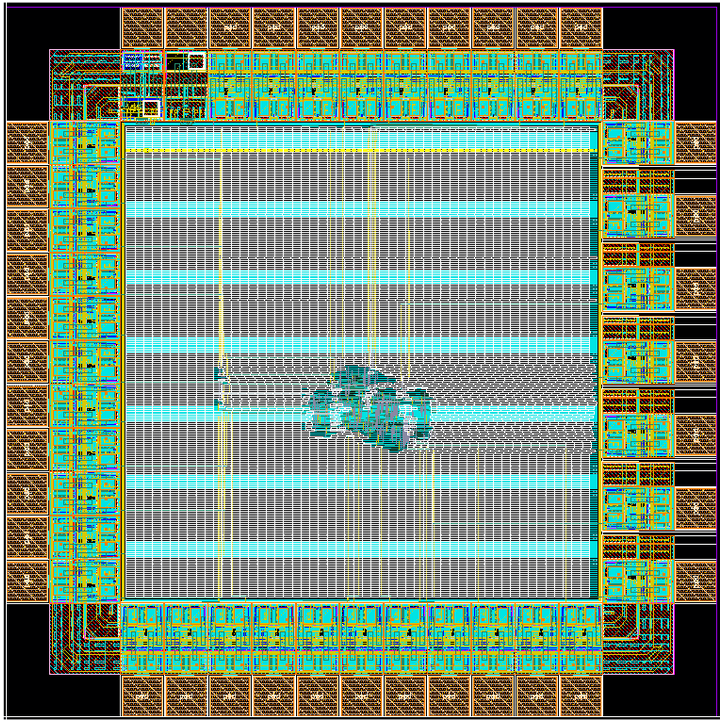
\includegraphics[width=0.5\textwidth]{images/chip.png}
\caption{The fully implemented design of the ECAU}
\label{chip}
\end{figure}

% Waveform
\begin{figure}%[H]
\centering
\captionsetup{justification=centering}
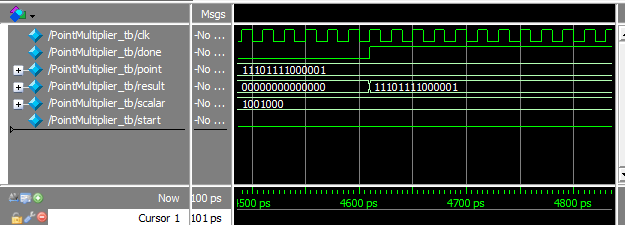
\includegraphics[width=0.5\textwidth]{images/simulation.png}
\caption{Multiplying a point on the curve by an arbitrary scalar}
\label{sim}
\end{figure}


The specifications of the chip can be seen in the table below:

 \begin{tabular}{ l l }
  Area Without Pads & 26083 ${\mu}m^2$ \\
  Total Area With Pads & 1082023 ${\mu}m^2$ \\
  Maximum Clock Frequency & 125 $MHz$ \\
  Total Dynamic Power Consumption & 364.1495 ${\mu}W$\\
\end{tabular}

\section{Future Work}
Optimizing the inversion operation would yield the greatest benefit for increasing performance. Operating over a bigger finite field would dramatically increase security, and even better would be to create modules that work over arbitrary finite fields up to a large bit-size (say, 512 bits). Serial input/output would massively decrease the number of pins required. A fully-fleshed out cryptographic system that could perform key-generation, message-signing, and signature verification would be the ultimate goal.

\section{Conclusion}
The ECAU shows that elliptic curve cryptography can be done in hardware with decent performance. More work will need to be done to scale up and generalize the modules to work with real-world applications. 

\bibliographystyle{IEEEtran}
\bibliography{IEEEabrv,bib/ref}

\end{document}

% Cite this http://cacr.uwaterloo.ca/hac/about/chap14.pdf
